%Reporte de computacional
\documentclass{article}

\usepackage{hyperref}
\usepackage{amsmath}
\usepackage{amsthm}
\usepackage{amssymb}
\usepackage{graphicx}
\usepackage{ifxetex}
\ifxetex
\usepackage{fontspec}
\else
\usepackage[T1]{fontenc}
\usepackage[utf8]{inputec}
\usepackage{lmodern}
\fi







\begin{document}

\title{Medición de Propiedades Atmosfericas}

\author{Ramses Pacheco Ortiz}

\maketitle             

\section{Introduccion}
Esta actividad desarrollamos un poco mas el uso del lenguage de python,con sus  librerias y plataforma, que la actividad pasada.
Nos apoyamos con los datos de sondeos atmosféricos que organiza la Universidad de Wyoming, para realizar la actividad 3, en donde se llevo a cabo el analisis de datos de un pais y con ayuda de la libreria de python pandas, se procedio a graficar los datos con ciertas especificaciones ya sea presion con altura,humedad con altura,etc.




\section{Fundamentos}

Previamenten en la primera practica estudiamos sobre la atmosfera terrestre, pero ahora estudiaremos como funciona los sondeos atmosferericos y algunas otras caracteristicas sobre estos:

Un sondeo meteorológico es básicamente una recopilación en tiempo real de todas las variables meteorológicas de la atmósfera mediante el lanzamiento de un globo sonda lleno de sensores. Se lanza el globo sonda desde la superficie, y, en su ascenso, va registrando todos los datos de la columna atmosférica: temperatura, humedad, viento, etc. Estos datos, unidos a los datos de centenares de atrás sondas que se lanzan en diferentes localizaciones del planeta, ayudan a configurar un mapa en tiempo real de las condiciones atmosféricas.

Otro fundamento en que se baso esta actvidad y que esta relacionada a los sondeos son los globos meteorologicos
 es un globo aerostático (específicamente un tipo de globo de gran altitud), que eleva instrumentos en la atmósfera para suministrar información acerca de la presión atmosférica, la temperatura, y la humedad por medio de un pequeño aparato de medida desechable llamado radiosonda. Para obtener datos del viento, los globos meteorológicos pueden ser rastreados por radar, radiolocalización o sistemas de navegación (tales como basado en satélites Sistema de Posicionamiento Global también conocido como GPS).
 
 \section{Analisis de Datos}
 Nosotros tomamos nuestros datos apoyandonos en los sondeos meteorologicos realizados por la universidad de Wyoming,seleccionamos los dias 22 de junio y 22 de diciembre del año 2017 del pais de Riverton,descargamos los datos y las librerias panda,matplit de jupyter para comenzar el analisis siguiente:
 
 \begin{enumerate}
 \item Cargaremos a la memoria de trabajo las bibliotecas: Pandas (manejo de datos, 
Numpy (numerical python) y la biblioteca de gráficas Matplotlib para proceder a modificar nuestros archivos de datos.

\begin{figure}[ht!]
 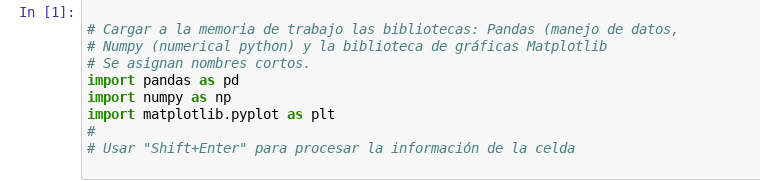
\includegraphics[width=1\linewidth]{3_1.png}
 \caption{Bibliotecas }
 \label{fig:1}
 \end{figure}
 
 \item Modificamos la lectura de los datos ya que en el archivo de texto que teniamos, leia unas comlumnas que no eran datos. Por eso le deimos la introduccion que no leiera los primeros 7 renglones del archivo de texto modificamos de la sigueinte manera:
 
 \begin{center}
	
    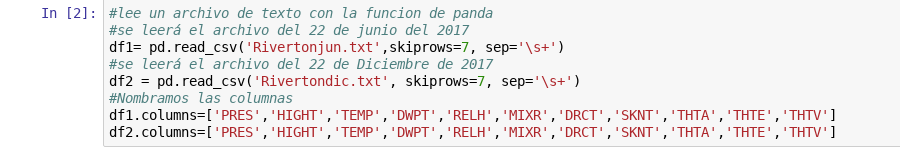
\includegraphics[height=2.5cm]{3_2.png}
\end{center}
 
 \item Realizamos una lectura de los datos de los que vamos a manejar utilizando la variable que contiene los datos con la modificacion vease las figuras.
 
 \begin{center}
	
    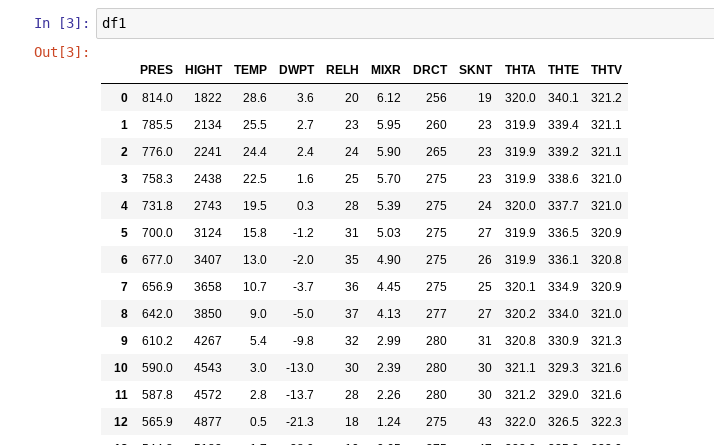
\includegraphics[height=8cm]{3_3.png}
\end{center}
 
 \begin{center}
	
    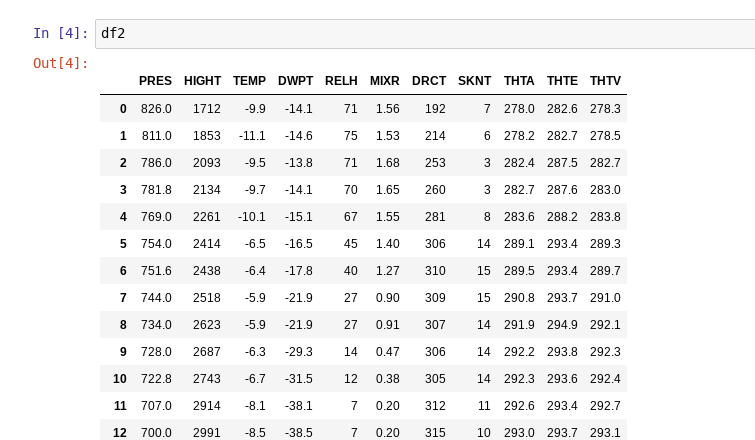
\includegraphics[height=8cm]{3_4.png}
\end{center}
 
 \item Lo siguiente que realizamos fue analizar los tipos de datos que teniamos
 
\begin{center}
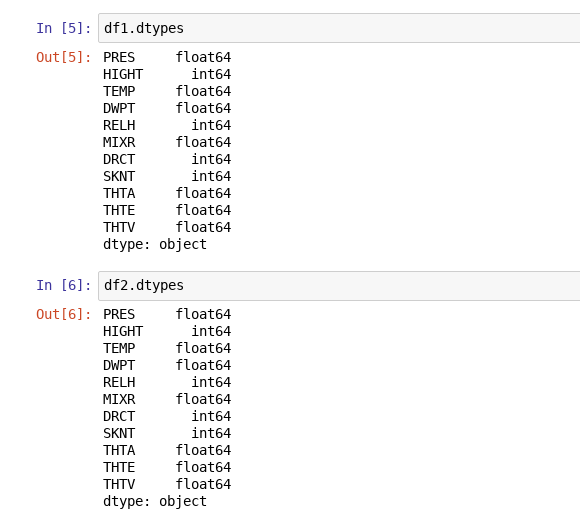
\includegraphics[height=10cm]{3_5.png}
\end{center}
 
 
 
 \end{enumerate}
 
 
 \section{Resultados}
 Para la presentacion de las graficas realziadas en la actvidad se mostrara el codigo y la grafica de los doms meses(junio y diciembre),considere que en cada una de esas graficas se llevaron acabo ciertos a justes de limites para que la graficas se vea bien.

\begin{itemize}
\item
 Las primeras graficas muestran la variación de la presión con la altura,Notemos que la presion disminuye conferme nos alejamos de la tierra.
 
 
 \begin{center}
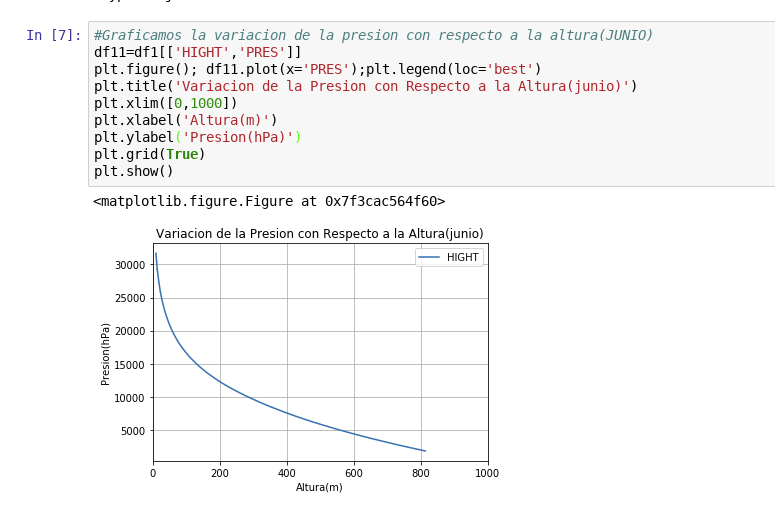
\includegraphics[height=7cm]{3_6.png}
\end{center}


\begin{center}
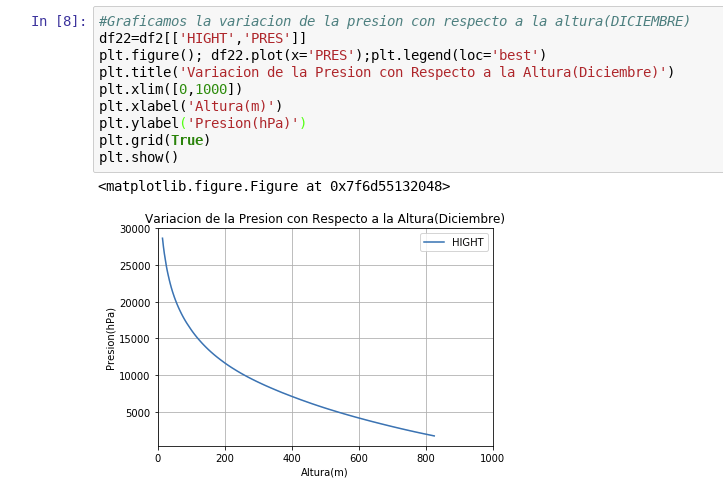
\includegraphics[height=7cm]{3_7.png}
\end{center}
 
 
 \item
 Las siguientes graficas y muestran la variacion de la temperatura contra la altura.
 No tenemos que conforme aumentamos la altura desciende la temperatura.
 
 \begin{center}
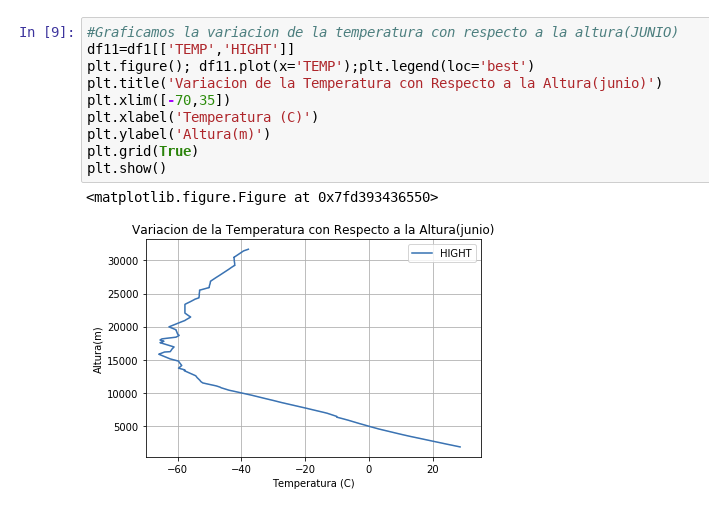
\includegraphics[height=7cm]{3_8.png}
\end{center}


\begin{center}
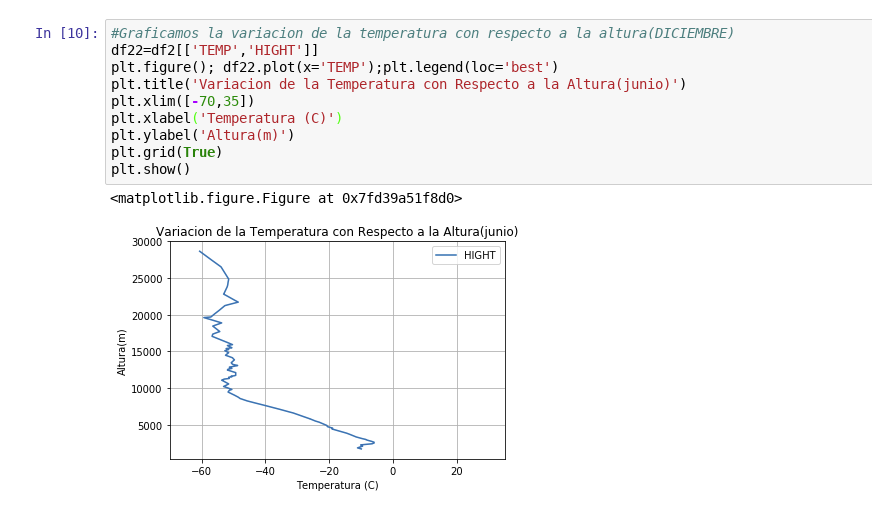
\includegraphics[height=7cm]{3_9.png}
\end{center}
 
 
 
 
 
 
 \item
 Las siguientes graficas muestran la variacion de la temperatura del rocío contra la altura.
Igual como en el caso anterior la temperatura del rocio desciende cuando la altura aumenta.
 
  \begin{center}
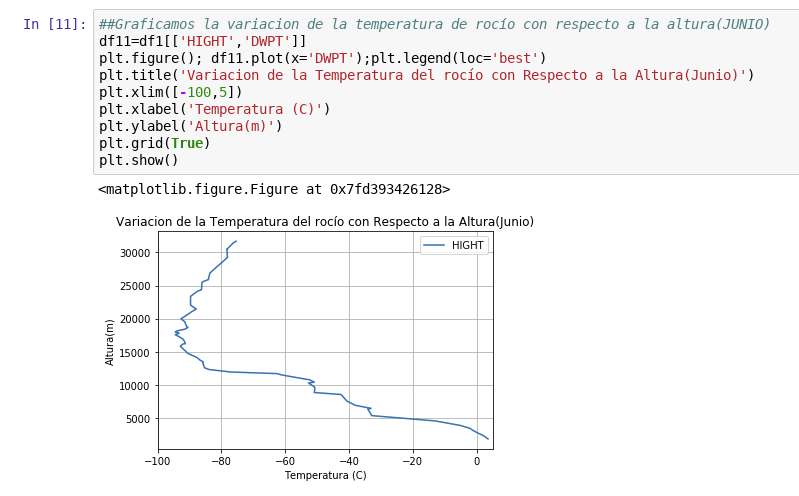
\includegraphics[height=7cm]{3_10.png}
\end{center}


\begin{center}
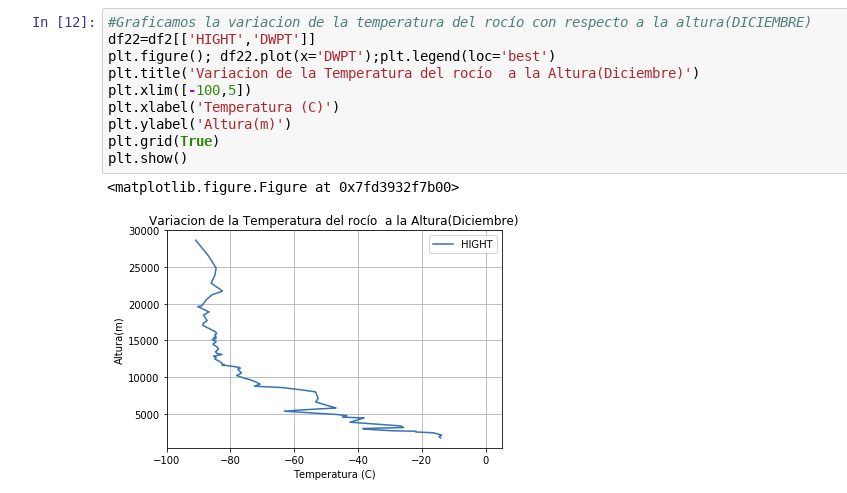
\includegraphics[height=7cm]{3_11.png}
\end{center}
 
 
 
 \item
 Las siguientes graficas muestran la variacion de la rapidez de los vientos en nudos. Como se observara varia un poco las velcidades de los veientos en ambos meses.
 
\begin{center}
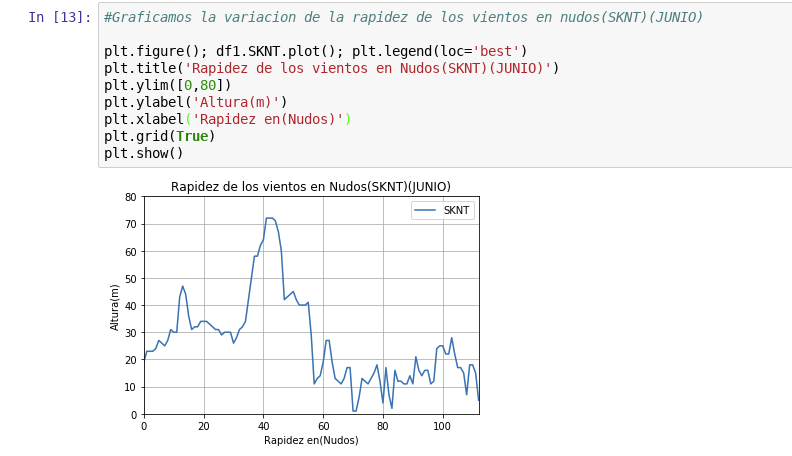
\includegraphics[height=7cm]{3_16.png}
\end{center}


\begin{center}
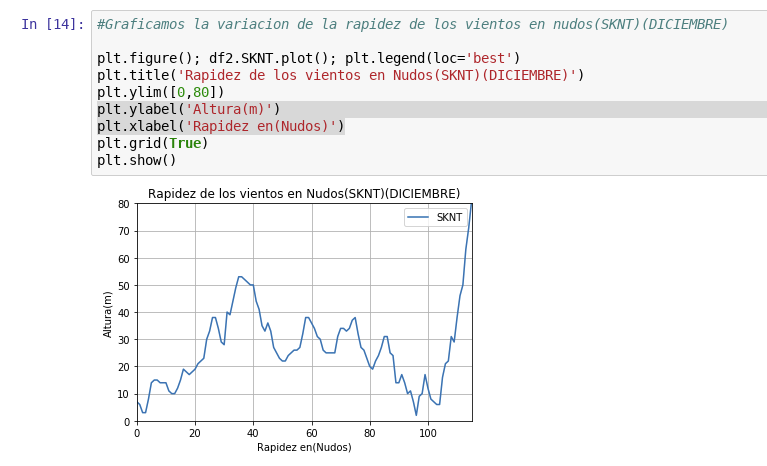
\includegraphics[height=7cm]{3_17.png}
\end{center}
 
 
 \item
 Las siguientes graficas muestran la variacion de la rapidez de los vientos en nudos. como observaran no varia mucho la humedad con respecto a la altura.
 
  \begin{center}
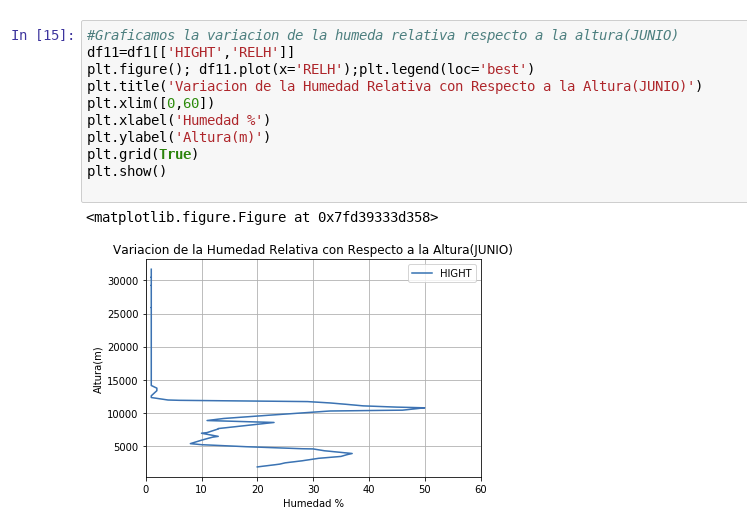
\includegraphics[height=7cm]{3_14.png}
\end{center}


\begin{center}
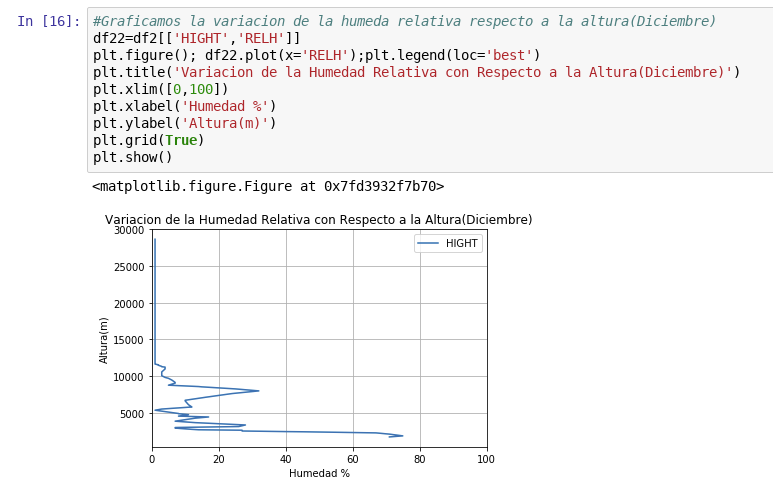
\includegraphics[height=7cm]{3_15.png}
\end{center}
 
 
 \section{Conclusion}
 
 Este trabajo al principio me paracio um poco facil, pero al momento de realizar las actividades se me complicaba el codigo de graficación, debido a los datos.
 
En cuanto a la teoria de la actividad me paracio muy intersante ya que conocimos un poco sobre los fenomenos de la naturaleza que ocurrian en dicho pais seleccionado.

\section{Bibliografia}
\item 
Atmospheric sounding. (2018).:
En.wikipedia.org. Recuperado el 13 de Febrero de 2018
desde, $https://en.wikipedia.org/wiki/Atmospheric_sounding$


\section{Apéndice}
\item\textbf{{¿Cuál es tu opinión general de esta actividad?}}

Me gusto mucho ya que reforce el conocimiento que tenia sobre la realziación de las graficas y las bibliotecas de panda 

\item\textbf{{¿Qué fue lo que más te agradó?}}

La elaboración de las graficas,ya que aprendi mas de como elaborar graficas.


\item\textbf{{¿Lo que menos te agradó?}}
Ninguna cosa, debido a que aprendi mucho.


\item\textbf{{¿Que consideras que aprendiste en esta actividad?}}

Como escribir el codigo para llevar acabo la grafica con los ciertos datos que necesites.

\item\textbf{{¿Qué le faltó? o ¿O le sobró?}}

Yo creo que esta muy completa la actividad.




    
 
\end{itemize}
 
  
 


\end{document}
